%%
%% This is file `sample-acmtog.tex',
%% generated with the docstrip utility.
%%
%% The original source files were:
%%
%% samples.dtx  (with options: `acmtog')
%% 
%% IMPORTANT NOTICE:
%% 
%% For the copyright see the source file.
%% 
%% Any modified versions of this file must be renamed
%% with new filenames distinct from sample-acmtog.tex.
%% 
%% For distribution of the original source see the terms
%% for copying and modification in the file samples.dtx.
%% 
%% This generated file may be distributed as long as the
%% original source files, as listed above, are part of the
%% same distribution. (The sources need not necessarily be
%% in the same archive or directory.)
%%
%% The first command in your LaTeX source must be the \documentclass command.
\documentclass[acmtog]{acmart}
%% NOTE that a single column version is required for 
%% submission and peer review. This can be done by changing
%% the \doucmentclass[...]{acmart} in this template to 
%% \documentclass[manuscript,screen]{acmart}
%% 
%% To ensure 100% compatibility, please check the white list of
%% approved LaTeX packages to be used with the Master Article Template at
%% https://www.acm.org/publications/taps/whitelist-of-latex-packages 
%% before creating your document. The white list page provides 
%% information on how to submit additional LaTeX packages for 
%% review and adoption.
%% Fonts used in the template cannot be substituted; margin 
%% adjustments are not allowed.

%%
%% \BibTeX command to typeset BibTeX logo in the docs
\usepackage{caption}
\usepackage{subcaption}
\usepackage{todonotes}
\usepackage{amsmath}
\usepackage{url}
\bibliographystyle{abbrvnat}

\settopmatter{printacmref=false}
\setcopyright{none}
\renewcommand\footnotetextcopyrightpermission[1]{} % removes footnote with conference information in first column

\AtBeginDocument{%
	\providecommand\BibTeX{{%
			\normalfont B\kern-0.5em{\scshape i\kern-0.25em b}\kern-0.8em\TeX}}}


%%
%% These commands are for a JOURNAL article.
\acmJournal{TOG}
\acmVolume{1}
\acmNumber{1}
\acmArticle{1}
\acmMonth{9}

%%
%% Submission ID.
%% Use this when submitting an article to a sponsored event. You'll
%% receive a unique submission ID from the organizers
%% of the event, and this ID should be used as the parameter to this command.
%%\acmSubmissionID{123-A56-BU3}

%%
%% The majority of ACM publications use numbered citations and
%% references.  The command \citestyle{authoryear} switches to the
%% "author year" style.
%%
%% If you are preparing content for an event
%% sponsored by ACM SIGGRAPH, you must use the "author year" style of
%% citations and references.
\citestyle{acmauthoryear}

%%
%% end of the preamble, start of the body of the document source.
\begin{document}
	
	%%
	%% The "title" command has an optional parameter,
	%% allowing the author to define a "short title" to be used in page headers.
	\title{Assignment 1}
	
	%%
	%% The "author" command and its associated commands are used to define
	%% the authors and their affiliations.
	%% Of note is the shared affiliation of the first two authors, and the
	%% "authornote" and "authornotemark" commands
	%% used to denote shared contribution to the research.
	
	\author{Casper Bresdahl}
	\affiliation{%
		\institution{whs715,}
		\institution{University of Copenhagen}
		\city{Copenhagen}
		\country{Denmark}}
	\email{whs715@alumni.ku.dk}
	
	%%
	%% By default, the full list of authors will be used in the page
	%% headers. Often, this list is too long, and will overlap
	%% other information printed in the page headers. This command allows
	%% the author to define a more concise list
	%% of authors' names for this purpose.
	%\renewcommand{\shortauthors}{Casper Bresdahl}
	
	%%
	%% The abstract is a short summary of the work to be presented in the
	%% article.
%	\begin{abstract}
%		Some abstract of my assignment goes here.
%	\end{abstract}
	
	\maketitle
	
	\section{Introduction}
This week we will first introduce the theory behind advection and mean curvature flow and how we can discretize these. We will then look at the first experiment looking into how advection without any boundary issues behave compared to advection where boundaries will play a role. We will then look at the second experiment where we will compare three different boundary conditions and how these change the end result when applying mean curvature flow to a signed distance field. At the end we will conclude on our results.
	\section{The Radon transform}
The \textit{Radon transform} defines projections of an object mapping it from its spatial domain to its projection space. That is, using the Radon transform on a 2D object from a single angle, we obtain a 1D projection of the object which can be interpreted as a histogram of the objects density from that angle. Having a 2D object, $f(x,y)$, defined in the spatial domain and the rectangular coordinate system, the Radon transform is defined as the projection $(p,\theta)$ in the polar coordinate system:
\begin{equation} \label{linearity}
	P(p,\theta) = \mathbf{R}\{f(x,y)\} = \int_L f(x,y) dl
\end{equation}  
Where $\int_L$ is the line integral defined along the path \textit{L}, such that $xcos(\theta) + ysin(\theta) = p$. The polar coordinate system, $(p,\theta)$, can be translated into rectangular coordinates by using a rotated coordinate system $(p,q)$ where:
\begin{align*}
	xcos(\theta) + ysin(\theta) &= p \\
	-xsin(\theta) + ycos(\theta) & = q
\end{align*}
This change of coordinates implies an equivalent definition of the Radon transform in terms of polar coordinates:
\begin{equation*}
	\mathbf{R}\{f(x,y)\} = \int_{-\infty}^{\infty}f(pcos(\theta) - qsin(\theta),psin(\theta)+qcos(\theta))dq
\end{equation*}
For a fixed angle $\theta$ the 1D function $P_{\theta}(p) = P(p,\theta)$ and is called a projection. It contains all line integrals over $f(x,y)$ with the constant angle $\theta$ and variable distance $p$ to the origin, and as described earlier, can be interpreted as a histogram of the objects density from this angle.\\
\begin{figure}
	\centering
	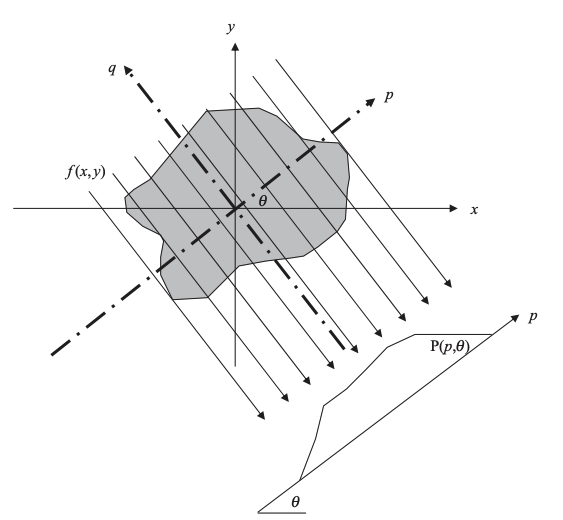
\includegraphics[width=\linewidth]{Materials/Projection}
	\caption{2D object $f(x,y)$ shown as shaded object in the rectangular coordinate system $(x,y)$. The lines indicate the direction the line integrals are computed, and are defined by the angle $\theta$ and sampled along the $p$ axis from the rotated coordinate system $(p,q)$. As a result of computing the line integrals, we see the 1D projection $P(p,\theta)$ in the bottom of the image. Image is from \cite{MIA}.}
	\label{projection}
\end{figure}
In \autoref{projection} we see a projection of a 2D object. We see the shaded object defined in the rectangular coordinate system $(x,y)$ and the lines for which the line integrals are taken along. The lines are defined by the angle $\theta$, and by taking the line integrals from $-\infty$ to $\infty$ we get the projection seen in the lower right of the image. We see how a 'high response' is measured when the object is wide along the lines, and a 'low response' when the object is narrow.\\
If we take the Radon transform over several angles we can concatenate the produced projections and construct a \textit{sinogram}. A sinogram has the angles sampled along the $x-axis$ and the distances $p$ along the $y-axis$. In \autoref{sino} we see a sinogram computed over a uniform circle. As the circle is not centered at the origin, the sinogram gets a curved shape because as we rotate around the circle the relative position to the projection plane shifts.

\begin{figure}
	\centering
	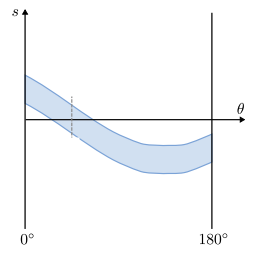
\includegraphics[width=0.5\linewidth]{Materials/sino}
	\caption{A sinogram computed over a uniform circle. Image from \cite{MIA}.}
	\label{sino}
\end{figure}
	\section{Understanding how the Radon transform is performed}
With the theory in place, we can now move on and look at some more practical applications of the Radon transform. In python we can use the \textit{skimage} library to perform the Radon transform on images. In \autoref{shepp} we see the Shepp-Logan phantom which is a common test image. It is composed of several ovals with varying uniform intensity. The result of taking the Radon transform of this image can be seen in \autoref{sheppSinoHighRes}. The result is at first glance hard to interpret, as it would seem to be a lot of sinus waves laid on top of each other, and thus we will begin by analysing some simpler shapes and their sinograms, and then return to the Shepp-Logan image when we have a greater understanding.\\
\begin{figure}
	\centering
	\begin{subfigure}{0.48\linewidth}
		\centering
		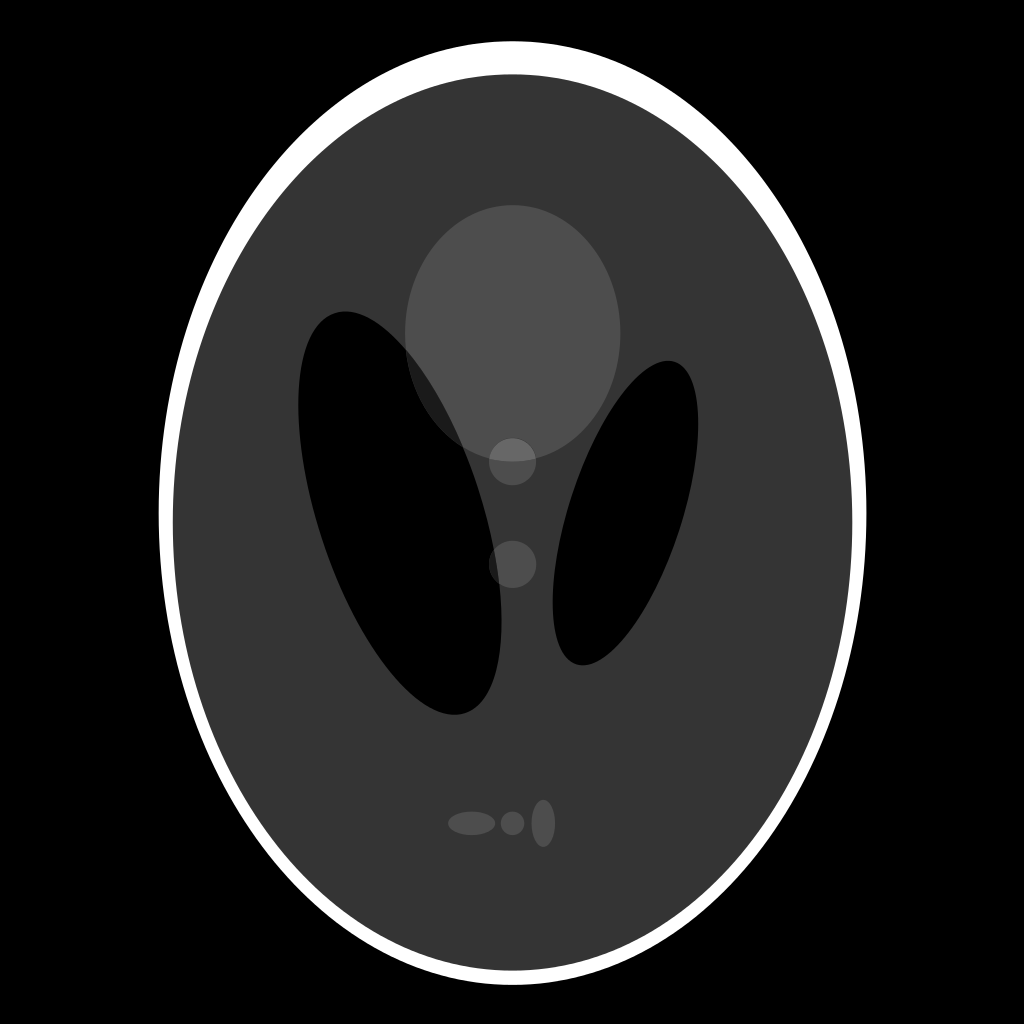
\includegraphics[width=\linewidth]{Materials/sheppLogan}
		\caption{The Shepp-Logan phantom.\newline\newline}
		\label{shepp}
	\end{subfigure}
	\hfill
	\begin{subfigure}{0.48\linewidth}
			\centering
			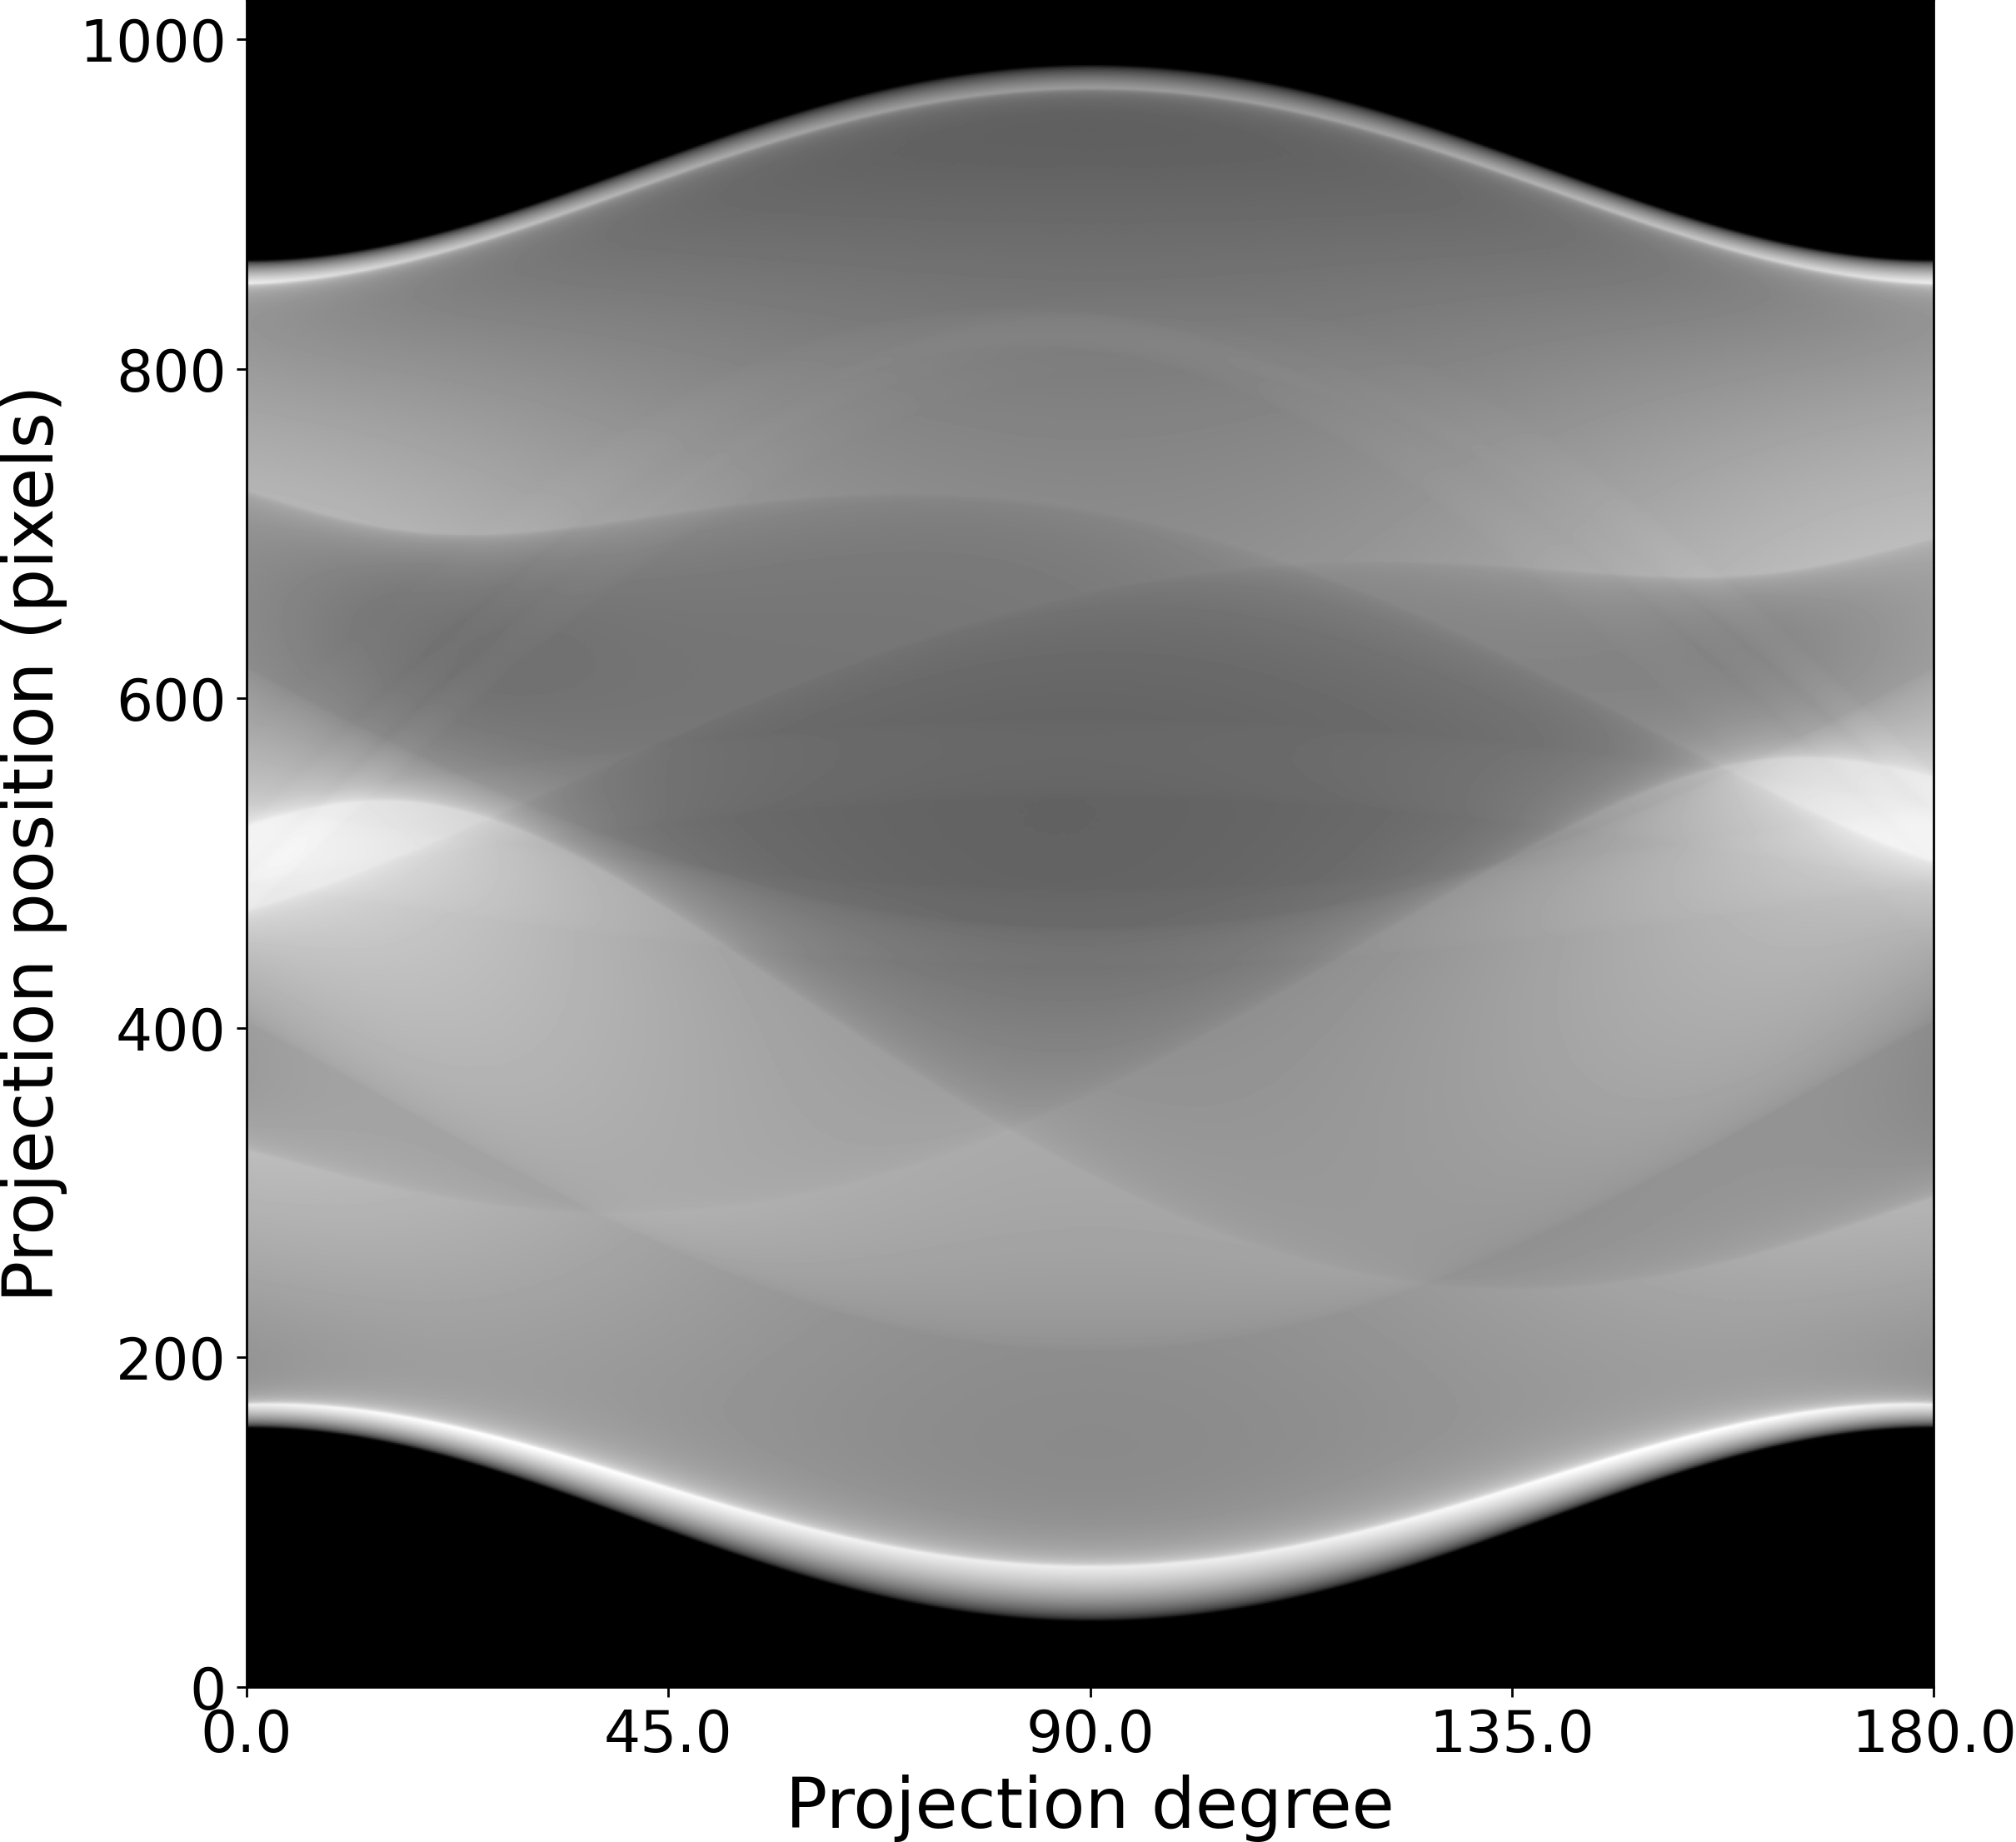
\includegraphics[width=\linewidth]{Materials/sheppLoganHighRes}
			\caption{Sinogram of The Shepp-Logan phantom taken with 1024 angles between 0 and 180 degrees.}
			\label{sheppSinoHighRes}
	\end{subfigure}
	\caption{The Shepp-Logan phantom along its sinogram computed over 180 degrees.}
\end{figure}
\begin{figure}
	\centering
	\begin{subfigure}{0.48\linewidth}
		\centering
		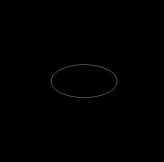
\includegraphics[width=\linewidth]{Materials/hEllipse}
		\caption{A vertical ellipse.\newline\newline}
		\label{hEllipse}
	\end{subfigure}
	\hfill
	\begin{subfigure}{0.48\linewidth}
		\centering
		
\includegraphics[height=1.5\linewidth]{Materials/hEllipseSino}
		\caption{Sinogram of a vertical ellipse taken with 180 angles between 0 and 180 degrees.}
		\label{hEllipseSino}
	\end{subfigure}
	\caption{A vertical ellipse and its sinogram.}
\end{figure}
In \autoref{hEllipse} we have drawn a simple vertical ellipse. Taking its sinogram we get the hourglass-shape seen in \autoref{hEllipseSino}. Thinking back to the theory, the sinograms are composed of several projections of the original object taken from several angles. In \autoref{hEllipseSino} we see the sinogram begins with a wide shape which then gets more narrow before it gets wide again. Based on these observations we can conclude the radon transform is initialized from either the top or the bottom of the original image.\\
\begin{figure}
	\centering
	\begin{subfigure}{0.48\linewidth}
		\centering
		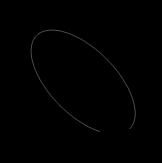
\includegraphics[width=\linewidth]{Materials/tEllipse}
		\caption{A slightly tilted ellipse.\newline\newline}
		\label{tEllipse}
	\end{subfigure}
	\hfill
	\begin{subfigure}{0.48\linewidth}
		\centering
		
\includegraphics[height=1.5\linewidth]{Materials/tEllipseSino}
		\caption{Sinogram of a slightly tilted ellipse taken with 180 angles between 0 and 180 degrees.}
		\label{tEllipseSino}
	\end{subfigure}
	\caption{A tilted ellipse and its sinogram.}
\end{figure}
In \autoref{tEllipse} we have tilted the ellipse slightly and in \autoref{tEllipseSino} we have its sinogram. We here see a shift in the narrow part as it now lies more to the left in the sinogram. This observation tells us we move in a counter clockwise motion around the original image when we do the Radon transform, as the narrow part of the ellipse is encountered first when starting either from the top or bottom and then moving counter clockwise around it.\\
As we now know we either start from the top or the bottom of the original image, and we move counter clockwise around it, we can now return to the sinogram of the Shepp-Logan image in \autoref{sheppSinoHighRes}. We note this sinogram is considerably more square than the other sinograms. This is due to the more angles used to obtain the sinogram. In the ellipses 180 angles between 0 and 180 degrees are used. This means each pixel column corresponds to a 1 degree turn. In the Shepp-Logan sinogram 1024 angles are used between 0 and 180 degrees. This means each pixel row is less than a 1 degree turn, however, we still begin at 0 degrees and end at 180 degrees, so end points of the images have the same relative meaning. Now looking at the middle part the of \autoref{sheppSinoHighRes} we see two darker shades, one being narrow and growing wider while moving from the top to the bottom, and one starting wide and growing narrow while moving from the bottom to the top. These two shades are the two big black ellipses in the middle of the Shepp-Logan phantom (\autoref{shepp}). We see this mainly because these are the darkest parts of the Shepp-Logan phantom, and so they will contribute with a low to no response in the sinogram, but we can also see based on our previous observations they behave as expected, as we begin the sinogram from either the top or bottom of the original image and move counter clockwise around it. As the two ellipses are slightly tilted to the opposite directions, we can actually determine that the sinogram is begun from the bottom, as the bigger of the dark shades in the sinogram begins in the top (left in the projection) in the sinogram and ends at the bottom (to the right in the projection). Had the Radon transform been begun from the top, we would have had seen the opposite.\\
But why have we chosen to only show 180 degrees? In \autoref{shepp360} we see a sinogram of the Shepp-Logan image taken from 1024 angles between 0 and 360 degrees. We here see a strong similarity to the 180 degrees sinogram in \autoref{sheppHighRes}, in fact, the first half (the first 180 degrees) is the same and the second is simply the first half mirrored. This also intuitively makes sense as the line integrals measure the intensities in the image 'the whole way through', and so, taking the sinogram from 180 degrees to 360 degrees gives the same response as from 0 to 180 degrees, simply mirrored in the \textit{x-axis}.
\begin{figure}
	\centering
	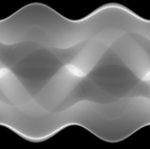
\includegraphics[width=0.5\linewidth]{Materials/shepp360}
	\caption{Sinogram of the Shepp-Logan image with 1024 angles between 0 and 360 degrees.}
	\label{shepp360}
\end{figure}
	\section{Linearity of the Radon transform}
It can be shown that the Radon transform is a linear transformation. By using the definition of \autoref{linearity} we can show:
\begin{align}
	\mathbf{R}\{\alpha f(x,y) + \beta g(x',y')\} &= \int_L \left(\alpha f(x,y) + \beta g(x',y')\right) dl\\
	&= \int_L \alpha f(x,y) dl + \int_L \beta g(x',y') dl \label{sumRule}\\
	&= \alpha \int_L f(x,y) dl + \beta \int_L g(x',y') dl \label{constantRule}\\
	&= \alpha \mathbf{R}\{f(x,y)\} + \beta \mathbf{R}\{g(x',y')\}
\end{align}
Where the sum rule is used in \autoref{sumRule} and the constant rule is used in \autoref{constantRule}. This shows the Radon transform is linear, and means adding two functions together and then taking the Radon transform is the same as taking the Radon transform and then adding the results together. This comes down to the line integrals used to achieve the projections. As images are discrete we can not comply exactly to the mathematical definitions with line integrals. Instead we can use a Riemann sum to approximate the line integrals, that is we can take the sum of pixel intensities along a line to approximate the line integrals. If we then take \autoref{linearityExplained} as an example, we have two uniform circles. If we imagine one is defined by $f(x,y)$ and the other by $g(x',y')$, then adding $f(x,y)$ and $g(x',y')$ together gives us \autoref{linearityExplained}. We can now quite intuitively see that taking the sum of pixel intensities along the lines shown \autoref{linearityExplained}, i.e. summing over the lines in $f(x,y) + g(x',y')$, would be the same as summing over the lines in first $f(x,y)$, then $g(x',y')$ and then finally add the results together.
\begin{figure}
	\centering
	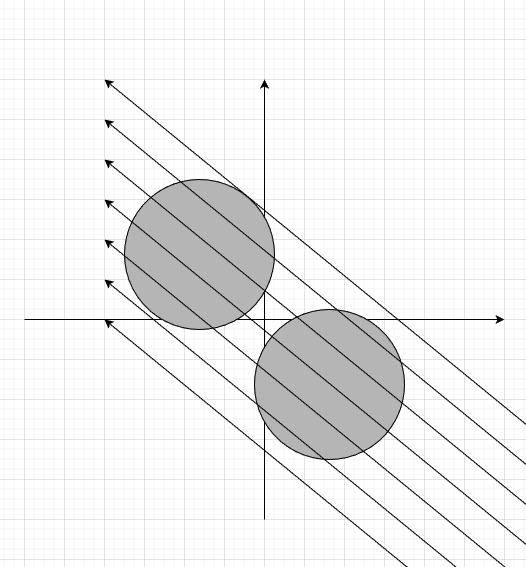
\includegraphics[width=\linewidth]{Materials/linearityExplained}
	\caption{Two uniform circles and the lines along which the line integrals are taken.}
	\label{linearityExplained}
\end{figure}
	\section{Back projection and filtered back projection}
One can now ask if it is possible to go back from a sinogram to an image, and in fact it is. Two common image reconstruction techniques which can be applied if a sinogram is obtained is back projection and filtered back projection. With back projection the response measured from the obtained projections are uniformly distributed back along the lines the line integrals were computed. Doing this for several projections results in areas where the reconstructed image will get more exposure, and thus a rough / blurred outline will appear. This is sketched in \autoref{backprojection} where we see object A and B would emerge in the reconstruction because the obtained responses from the projections will intersect at these locations. A back projection can be seen in \autoref{reconbackprojection}.\\
\begin{figure}
	\centering
	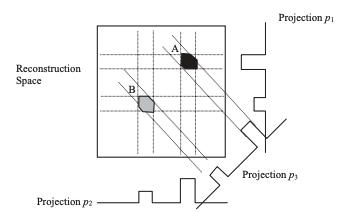
\includegraphics[width=0.9\linewidth]{Materials/backprojection}
	\caption{Illustration of back projection. By uniformly distribute the response from the obtained projections back along the line it was obtained a blurred reconstruction can be obtained. Image taken from \cite{MIA}.}
	\label{backprojection}
\end{figure}
\begin{figure}
	\centering
	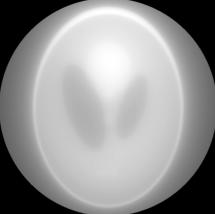
\includegraphics[width=0.6\linewidth]{Materials/reconnofilter}
	\caption{Result of a back projection made with the library \textit{skimage} setting the \textit{filter} parameter of the \textit{iradon} function to 'None'.}
	\label{reconbackprojection}
\end{figure}
To achieve sharper results, the filtered back projection is used. In filtered back projection the obtained projections are taken into frequency space by computing the 1D Fourier transform. The Fourier Slice Theorem then establishes a relationship between $F(u,v) = \mathcal{F}\{f(x,y)\}$ and $P(\mathcal{E},\theta) = \mathcal{F}\{p_{\theta}(p)\}$ where $P(\mathcal{E},\theta)$ is equivalent to the part of $F(u,v)$ that falls on a radial line with angle $\theta$. That is, by computing the Fourier transform of the 1D projections and using the Fourier Slice Theorem, we obtain a single line in 2D frequency space. By adding several projections together in this way we end with a 'filled' frequency space and we can then take the 2D inverse Fourier transform and get an approximation to the original function $f(x,y)$. In \autoref{filteredbackprojection} an outline of this process is sketched.\\
\begin{figure}
	\centering
	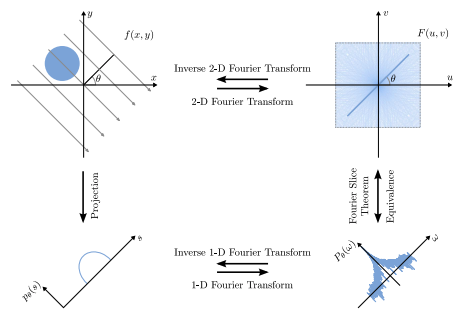
\includegraphics[width=\linewidth]{Materials/filteredbackprojection}
	\caption{Illustration of filtered back projection. First a projection is made, the its Fourier transform is computed. The Fourier Slice Theorem is then used to bring the 1D signal into a 2D line. Several lines can then be added together to 'fill' the frequency space. Finally an inverse Fourier transform can then be used to approximate the original function. Image taken from \cite{MIS}.}
	\label{filteredbackprojection}
\end{figure}
A slight issue to simply implement this pipeline is, the further out towards the endpoints of the lines in the frequency space we go, i.e. the more frequencies we include, the further the distance becomes between the lines, and thus the less information we have. To get more information one could simply sample more lines, i.e. obtain more projections, however, this would both be time consuming and expose the patient for more radioactivity. Instead one can limit the frequencies used by simply doing a cutoff at a certain 'max frequency'. However, as all the lines always will go through the origin, the lower frequencies are likely to be over represented. A Ram-Lak filter, shown in \autoref{ramlak}, is thus often used. This filter suppresses low frequencies while amplifying high, under sampled, frequencies, while providing a cutoff at some max frequency. Using the filter is also cheap in terms of efficiency as we are already in frequency space where a multiplication with the Ram-Lak filter will result in a convolution with it in the spacial domain.\\
\begin{figure}
	\centering
	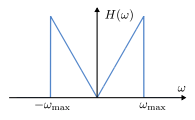
\includegraphics[width=0.7\linewidth]{Materials/RamLak}
	\caption{The Ram-Lak filter. Image taken from \cite{MIS}.}
	\label{ramlak}
\end{figure}
A common use case for filtered back projection is CT reconstruction, where after the CT scan one gets a number of projections which then can be used to approximate the original object scanned. 
	\section{Reconstruction results}
We will now take a look at some image reconstructions obtained by performing filtered back projection. This has been done in python with the \textit{skimage} library.\\
\begin{figure}
	\centering
	\begin{subfigure}{0.48\linewidth}
		\centering
		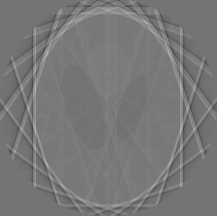
\includegraphics[width=\linewidth]{Materials/recon10}
		\caption{Reconstruction of the Shepp-Logan phantom with 10 angles taken between 0 and 180 degrees.}
	\end{subfigure}
	\hfill
	\begin{subfigure}{0.48\linewidth}
		\centering
		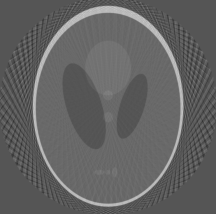
\includegraphics[width=\linewidth]{Materials/recon45}
		\caption{Reconstruction of the Shepp-Logan phantom with 45 angles taken between 0 and 180 degrees.}
	\end{subfigure}
	\\
	\begin{subfigure}{0.48\linewidth}
		\centering
		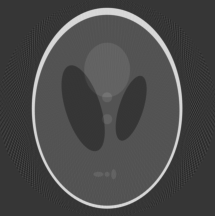
\includegraphics[width=\linewidth]{Materials/recon100}
		\caption{Reconstruction of the Shepp-Logan phantom with 100 angles taken between 0 and 180 degrees.}
	\end{subfigure}
	\hfill
	\begin{subfigure}{0.48\linewidth}
		\centering
		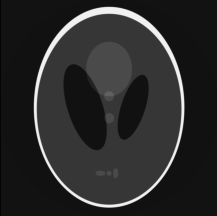
\includegraphics[width=\linewidth]{Materials/recon360}
		\caption{Reconstruction of the Shepp-Logan phantom with 360 angles taken between 0 and 180 degrees.}
	\end{subfigure}
	\caption{Reconstructions of the Shepp-Logan phantom with varying number of projections used.}
	\label{recons}
\end{figure}
In \autoref{recons} we see four image reconstructions of the Shepp-Logan phantom where we have used a varying number of projections to achieve the reconstruction. We see with only 10 projections the most prominent features, namely the big white oval and the two darker ovals in the middle, are reconstructed. However, we also see big artefacts. Using 45 projections we obtain all features of the original image, however, the reconstruction still has a lot of artefacts now seen as a chequerboard patterns around the reconstructed object. Using 100 projections we now have almost no artefacts, and the reconstruction is almost identical to the original image, just brighter and slightly blurred. With 360 projections the artefacts seems to be gone and the reconstruction is \textit{very} close to the original the only differences is the reconstruction is \textit{slightly} blurred and a bit brighter.\\
Comparing \autoref{reconbackprojection} and the reconstructions in \autoref{recons} we see a huge improvement in sharpness and detail.\\
The filtered back projection is a linear reconstruction technique, and thus we can also achieve a complete reconstruction from a sum of reconstructions. By constructing four reconstructions, each consisting of 45 angles, and having them reconstruct one quadrant each, i.e. the first reconstructs 0-45 degrees, the second 45-90 degrees and so on, we can achieve a complete reconstructions by summing the results. The partial reconstructions can be seen in \autoref{partials} and the complete reconstruction can be seen in \autoref{complete}. We see the complete reconstruction is practically identically with the reconstruction obtained in \autoref{recons} where 360 angles were used.
\begin{figure}
	\centering
	\begin{subfigure}{0.48\linewidth}
		\centering
		
\includegraphics[width=\linewidth]{Materials/lin1}
		\caption{Reconstruction of the Shepp-Logan phantom with 45 angles taken between 0 and 45 degrees.}
	\end{subfigure}
	\hfill
	\begin{subfigure}{0.48\linewidth}
		\centering
		
\includegraphics[width=\linewidth]{Materials/lin2}
		\caption{Reconstruction of the Shepp-Logan phantom with 45 angles taken between 45 and 90 degrees.}
	\end{subfigure}
	\\
	\begin{subfigure}{0.48\linewidth}
		\centering
		
\includegraphics[width=\linewidth]{Materials/lin3}
		\caption{Reconstruction of the Shepp-Logan phantom with 45 angles taken between 90 and 135 degrees.}
	\end{subfigure}
	\hfill
	\begin{subfigure}{0.48\linewidth}
		\centering
		
\includegraphics[width=\linewidth]{Materials/lin4}
		\caption{Reconstruction of the Shepp-Logan phantom with 45 angles taken between 135 and 180 degrees.}
	\end{subfigure}
	\caption{Reconstructions of the Shepp-Logan phantom each a reconstruction of a quadrant.}
	\label{partials}
\end{figure}
\begin{figure}
	\centering
	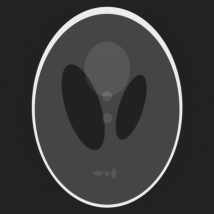
\includegraphics[width=0.5\linewidth]{Materials/complete}
	\caption{The complete reconstruction obtained by adding the four partial reconstructions together.}
	\label{complete}
\end{figure}
	\section{Conclusion}
In conclusion we have seen where segmentation can be used in medical image analysis, we have seen the risks of dilation and erosion and explained the benefits of them, we have concluded Graph cut segmentations are preferred, but also have limited applications and Random walker alleviates these constrains by being non-deterministic, and finally we have looked into how PCA can be used for segmentation.
	\newpage
	\bibliography{Exercises/bibliography}
	\newpage

	%\bibliography{Exercises/mybib}

	
\end{document}
\endinput
